\documentclass[handout]{beamer}
\iffalse

MIT License

Copyright (c) 2023-2025 Aron Hardeman

Permission is hereby granted, free of charge, to any person obtaining a copy
of this software and associated documentation files (the "Software"), to deal
in the Software without restriction, including without limitation the rights
to use, copy, modify, merge, publish, distribute, sublicense, and/or sell
copies of the Software, and to permit persons to whom the Software is
furnished to do so, subject to the following conditions:

The above copyright notice and this permission notice shall be included in all
copies or substantial portions of the Software.

THE SOFTWARE IS PROVIDED "AS IS", WITHOUT WARRANTY OF ANY KIND, EXPRESS OR
IMPLIED, INCLUDING BUT NOT LIMITED TO THE WARRANTIES OF MERCHANTABILITY,
FITNESS FOR A PARTICULAR PURPOSE AND NONINFRINGEMENT. IN NO EVENT SHALL THE
AUTHORS OR COPYRIGHT HOLDERS BE LIABLE FOR ANY CLAIM, DAMAGES OR OTHER
LIABILITY, WHETHER IN AN ACTION OF CONTRACT, TORT OR OTHERWISE, ARISING FROM,
OUT OF OR IN CONNECTION WITH THE SOFTWARE OR THE USE OR OTHER DEALINGS IN THE
SOFTWARE.

\fi
\usepackage[utf8]{inputenc}

\title{Calculus for CS+AI}
\author[Mihnea Pasere \& Aron Hardeman]{\texorpdfstring{Aron Hardeman \& Mihnea Pasere\\\textcolor{gray}{Slides by Aron Hardeman}}{Aron Hardeman}}
\date[March 27, 2025]{March 27, 2025\\This is an unofficial lecture organized by S.V. Cover.}

\usetheme{Madrid}
\usecolortheme{whale}
\useoutertheme[subsection=false]{miniframes}
\setbeamertemplate{section in toc shaded}[default][44]
\setbeamertemplate{subsection in toc shaded}[default][44]




\usepackage[utf8]{inputenc}
\usepackage{amssymb,amsmath}
\usepackage{tikz}
\usepackage{tikz-qtree}
\usepackage{color}
\usepackage{fancyhdr}
\usepackage{lplfitch}
\usepackage{fancyhdr}
\usepackage{graphicx}
\usepackage[most]{tcolorbox}
\usepackage{float}
\usepackage{natbib}
\usepackage{stmaryrd}
\usepackage{relsize}
\usepackage{tensor}
\usepackage{microtype}
\usepackage{pgfplots}
\usepgfplotslibrary{polar}
\usetikzlibrary{quotes,angles}
\usetikzlibrary{babel}
\usepackage{verbatim}
\pgfplotsset{width=8cm,compat=1.9}

\DeclareMathOperator{\atantwo}{atan2}
\DeclareMathOperator{\Arg}{Arg}


\begin{document}

\maketitle

%\iffalse

MIT License

Copyright (c) 2023 Aron Hardeman

Permission is hereby granted, free of charge, to any person obtaining a copy
of this software and associated documentation files (the "Software"), to deal
in the Software without restriction, including without limitation the rights
to use, copy, modify, merge, publish, distribute, sublicense, and/or sell
copies of the Software, and to permit persons to whom the Software is
furnished to do so, subject to the following conditions:

The above copyright notice and this permission notice shall be included in all
copies or substantial portions of the Software.

THE SOFTWARE IS PROVIDED "AS IS", WITHOUT WARRANTY OF ANY KIND, EXPRESS OR
IMPLIED, INCLUDING BUT NOT LIMITED TO THE WARRANTIES OF MERCHANTABILITY,
FITNESS FOR A PARTICULAR PURPOSE AND NONINFRINGEMENT. IN NO EVENT SHALL THE
AUTHORS OR COPYRIGHT HOLDERS BE LIABLE FOR ANY CLAIM, DAMAGES OR OTHER
LIABILITY, WHETHER IN AN ACTION OF CONTRACT, TORT OR OTHERWISE, ARISING FROM,
OUT OF OR IN CONNECTION WITH THE SOFTWARE OR THE USE OR OTHER DEALINGS IN THE
SOFTWARE.

\fi\section{Limits}
\tableofcontents[currentsection,currentsubsection]

\begin{frame}

\frametitle{Basic limits}

\begin{itemize}
\item  $\lim\limits_{x\to1}\frac{x^2-1}{x-1}=$\pause$\lim\limits_{x\to1}\frac{(x+1)(x-1)}{(x-1)}=\lim\limits_{x\to1}(x+1)=1+1=2$
\item\pause $\lim\limits_{t\to-4^-}\frac{x^2+9x+20}{\left|x+4\right|}=$\pause$\lim\limits_{t\to-4^-}\frac{x^2+9x+20}{-(x+4)}=\lim\limits_{t\to-4^-}\frac{(x+5)(x+4)}{-(x+4)}=\lim\limits_{t\to-4^-}-(x+5)=-(-4+5)=-1$
\item\pause $\lim\limits_{x\to-4}\frac{\sqrt{x^2+9}-5}{x+4}=$\pause$\lim\limits_{x\to-4}\frac{\sqrt{x^2+9}-5}{x+4}\cdot\frac{\sqrt{x^2+9}+5}{\sqrt{x^2+9}+5}=$
    \pause$\lim\limits_{x\to-4}\frac{x^2+9-25}{(x+4)(\sqrt{x^2+9}+5)}=$
    \pause$\lim\limits_{x\to-4}\frac{(x+4)(x-4)}{(x+4)(\sqrt{x^2+9}+5)}=$\pause$\lim\limits_{x\to-4}\frac{x-4}{\sqrt{x^2+9}+5}=\frac{-4-4}{\sqrt{(-4)^2+9}+5}=$\pause$~-\frac{4}{5}$
\end{itemize}


\end{frame}

\begin{frame}

\frametitle{L'Hôpital's rule}

\begin{tcolorbox}[colback=yellow!50,colframe=violet!85!black,title=L'Hôpital's rule]
    If we have a limit $\lim\limits_{x\to a}\frac{f(x)}{g(x)}$ \textbf{that is an indeterminate form of type $\pmb{\frac{0}{0}}$ or $\pmb{\frac{\infty}{\infty}}$}, then\footnote{\scriptsize if $f$ and $g$ are differentiable and $g'(x)\neq0$ in a neighborhood of $a$ (except possibly at $a$) and if $\lim\limits_{x\to a}\frac{f'(x)}{g'(x)}$ exists or is $\pm\infty$}, we have \[\lim\limits_{x\to a}\frac{f(x)}{g(x)}=\lim\limits_{x\to a}\frac{f'(x)}{g'(x)}\]

    
\end{tcolorbox}
\begin{itemize}
    \item $\lim\limits_{x\to0}\frac{2\sin x-\sin2x}{x-\sin x}=$\pause$\lim\limits_{x\to0}\frac{2\cos x-2\cos 2x}{1-\cos x}=$ \pause $\lim\limits_{x\to0}\frac{-2\sin x + 4\sin2x}{\sin x}=$ \pause $\lim\limits_{x\to0}\frac{-2\cos x + 8\cos2x}{\cos x}=$ \pause $\frac{-2+8}{1}=\boxed{6}$
\end{itemize}

\end{frame}


\begin{frame}

\frametitle{Squeeze theorem}

\begin{tcolorbox}[colback=yellow!50,colframe=violet!85!black,title=Squeeze theorem]
    If $f(x)\leq g(x)\leq h(x)$ for $x$ near $a$ (except possibly at $a$), then:

    \[\lim\limits_{x\to a}f(x)=\lim\limits_{x\to a}h(x)=L\quad\implies\quad \lim\limits_{x\to a}g(x)=L\]
    
\end{tcolorbox}
\begin{itemize}
    \item $\lim\limits_{x\to0}{x^{2}\sin\frac{1}{x}}=?$
    \item\pause We have $-1\leq\sin\frac{1}{x}\leq1$ for all real non-zero x, and $x^2\geq0$, thus also: $-x^2\leq x^2\sin\frac{1}{x}\leq x^2$
    \item\pause $\lim\limits_{x\to0}(-x^2)=\lim\limits_{x\to0}x^2=0$, therefore $\boxed{\lim\limits_{x\to0}x^2\sin\frac{1}{x}=0}$.
\end{itemize}

\end{frame}

\begin{frame}

\frametitle{Limits with $e$}

\begin{tcolorbox}[colback=yellow!50,colframe=violet!85!black,title=Euler's number]
    Euler's number is equal to $e=\lim\limits_{n\to\infty}\left(1+\frac{1}{n}\right)^n$.
    
\end{tcolorbox}
\begin{itemize}
    \item\pause Question: calculate $\lim\limits_{x\to\infty}\left(\frac{x+11}{x+5}\right)^{7x+3}$.
    \item\pause Solution: next slide.
\end{itemize}

\end{frame}

\begin{frame}{Example limit with $e$}
    \begin{align*}
        \action<+->{\hspace{-3mm}\lim\limits_{x\to\infty}&\left(\frac{x+11}{x+5}\right)^{7x+3}
        =}\action<+->{\lim\limits_{x\to\infty}\left(1+\frac{6}{x+5}\right)^{7x+3}
        =}\action<+->{\lim\limits_{x\to\infty}\left(1+\frac{1}{\frac{x}{6}+\frac{5}{6}}\right)^{7x+3}}\\
        \action<+->{\hspace{-3mm}&=\lim\limits_{x\to\infty}\left(1+\frac{1}{\frac{x}{6}+\frac{5}{6}}\right)^{\left(\frac{x}{6}+\frac{5}{6}\right)\cdot6\cdot7-35+3}
        =}\action<+->{\lim\limits_{x\to\infty}\left(1+\frac{1}{\frac{x}{6}+\frac{5}{6}}\right)^{\left(\frac{x}{6}+\frac{5}{6}\right)\cdot42-32}}\\
        \action<+->{\hspace{-3mm}&=\lim\limits_{x\to\infty}\left(\left(1+\frac{1}{\frac{x}{6}+\frac{5}{6}}\right)^{\left(\frac{x}{6}+\frac{5}{6}\right)}\right)^{42} \left(1+\frac{1}{\frac{x}{6}+\frac{5}{6}}\right)^{-32}}\\
        \action<+->{\hspace{-3mm}&=\left(\lim\limits_{x\to\infty}\left(1+\frac{1}{\frac{x}{6}+\frac{5}{6}}\right)^{\left(\frac{x}{6}+\frac{5}{6}\right)}\right)^{42} \cdot 1}\action<+->{=\boxed{\boxed{\mathlarger{\mathlarger{e^{42}}}}}}
    \end{align*}
\end{frame}

%\iffalse

MIT License

Copyright (c) 2023 Aron Hardeman

Permission is hereby granted, free of charge, to any person obtaining a copy
of this software and associated documentation files (the "Software"), to deal
in the Software without restriction, including without limitation the rights
to use, copy, modify, merge, publish, distribute, sublicense, and/or sell
copies of the Software, and to permit persons to whom the Software is
furnished to do so, subject to the following conditions:

The above copyright notice and this permission notice shall be included in all
copies or substantial portions of the Software.

THE SOFTWARE IS PROVIDED "AS IS", WITHOUT WARRANTY OF ANY KIND, EXPRESS OR
IMPLIED, INCLUDING BUT NOT LIMITED TO THE WARRANTIES OF MERCHANTABILITY,
FITNESS FOR A PARTICULAR PURPOSE AND NONINFRINGEMENT. IN NO EVENT SHALL THE
AUTHORS OR COPYRIGHT HOLDERS BE LIABLE FOR ANY CLAIM, DAMAGES OR OTHER
LIABILITY, WHETHER IN AN ACTION OF CONTRACT, TORT OR OTHERWISE, ARISING FROM,
OUT OF OR IN CONNECTION WITH THE SOFTWARE OR THE USE OR OTHER DEALINGS IN THE
SOFTWARE.

\fi
\section{Complex numbers}
\tableofcontents[currentsection,currentsubsection]
\begin{frame}
\frametitle{Basic arithmetic}

Complex numbers $(a+bi$ with $a,b\in\mathbb{R})$ behave just like you'd expect when doing simple arithmetic. For example:

\pause $(12-23i) + (3+6i) = 15 -17i$

\pause $(12-23i) - (3+6i) = 9 -29i$

\pause $(5+6i)(7+8i) = 35+82i+48i^2 = -13+82i$

\pause For division, use this trick with the complex conjugate of the denominator:

$\frac{2-3i}{4-5i}=$\pause$\frac{2-3i}{4-5i}\cdot\underbrace{\frac{4+5i}{4+5i}}_{=1} $\pause$= \frac{(2-3i)(4+5i)}{(4-5i)(4+5i)}$\pause$=\frac{23-2i}{41}$\pause$=\boxed{\frac{23}{41}-\frac{2}{41}i}$


\end{frame}

\begin{frame}
\frametitle{Complex plane}

Complex numbers lie in the \textit{complex plane}.

%\pause\includegraphics[scale=0.8]{plane.png}

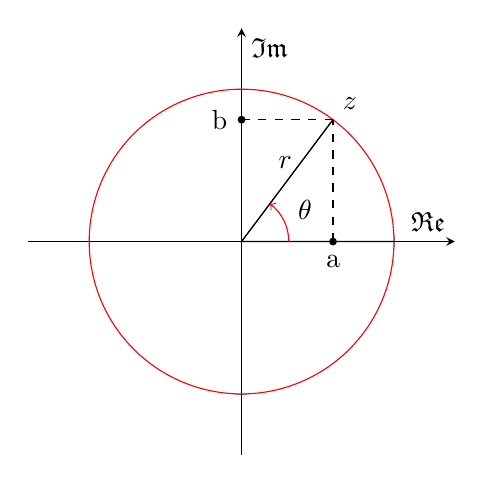
\begin{tikzpicture}
\begin{axis}[xlabel=$\mathfrak{Re}$,ylabel=$\mathfrak{Im}$,xmin=-7,ymin=-7,xmax=7,ymax=7,axis lines = middle,width=7cm,height=7cm,yticklabels={,,},xticklabels={,,}]
\addplot[data cs=polar,red,domain=0:360,samples=360,smooth] (x,5);
%\node[label={30:{(3,4)}},circle,fill,inner sep=2pt] at (axis cs:3,4) {};
\node[label={270:{a}},circle,fill,inner sep=1pt] at (axis cs:3,0) {};
\node[label={180:{b}},circle,fill,inner sep=1pt] at (axis cs:0,4) {};
\draw (axis cs:0,0) -- node[label={[xshift=0.1cm, yshift=-0.1cm]$r$}, left]{} (axis cs:3,4);
\draw[dashed] (axis cs:0,4) -- (axis cs:3,4);
\draw[dashed] (axis cs:3,0) -- (axis cs:3,4);
\draw
  (axis cs:5,0) coordinate (a)
  -- (axis cs:0,0) coordinate (b)
  -- (axis cs:3,4) coordinate (c) node[above right] {$z$}
  pic["$\theta$",draw=red,->,angle eccentricity=1.5,angle radius=0.6cm] {angle=a--b--c};
\end{axis}
\end{tikzpicture}
${\boxed{\boxed{z=a+bi=re^{i\theta}=r[\cos\theta+i\sin\theta]}}}$



\pause Instead of writing $a+bi$ (rectangular form), we can equivalently write $re^{i\theta}$ or $r[\cos\theta+i\sin\theta]$. The latter is known as the \textit{polar form}.
\end{frame}

\begin{frame}
\frametitle{Converting to exponential and polar form}
\begin{itemize}
\item The modulus of a complex number $z=x+yi$ is $\boxed{r=|z|=\sqrt{x^2+y^2}}$.

\item\pause In order to find the (principal) argument $\Arg(z)$, use the formula:
\[{\theta=\Arg(z)=\atantwo(y,x)=\begin{cases}
\arctan(\frac{y}{x}) &x>0\\
\arctan(\frac{y}{x})+\pi &x<0, y\geq0\\
\arctan(\frac{y}{x})-\pi &x<0, y<0 \\
\frac{\pi}{2}&x=0, y>0\\
-\frac{\pi}{2} &x=0, y<0\\
\text{(undefined)} &x=0, y=0
\end{cases}}\]

This formula gives the angle between $-\pi<\theta\leq\pi$.

\pause\textbf{Angles are in radians!} Fun fact: the function $\atantwo(y,x)$ is implemented in many programming languages, including C, Java, ...

\end{itemize}
\end{frame}

\begin{frame}{Converting to exponential form (examples)}
    \begin{itemize}
        \item\pause  $1+i=\sqrt{2}\cdot e^{i\pi/4}$ \textcolor{gray}{(since $\sqrt{1^2+1^2}=\sqrt{2}$ and $\Arg(1+i)=\frac{\pi}{4}$)}
        \item\pause  $1-i=\sqrt{2}\cdot e^{-i\pi/4}$ \textcolor{gray}{(now the angle is $\Arg(1-i)=-\frac{\pi}{4}$)}
        \item\pause  $-10=10e^{i\pi}$ \textcolor{gray}{($-10$ lies on the negative real axis, so the angle is $\pi$)}
    \end{itemize}

    
\end{frame}

\begin{frame}
\frametitle{Multiplying two complex numbers (polar form)}
\begin{itemize}
\item Suppose that we have two complex numbers $z_1=r_1 e^{i\theta_1}$ and $z_2=r_2 e^{i\theta_2}$. Let's see what happens when we multiply:
\pause\item $z_1z_2=r_1e^{i\theta_1}r_2 e^{i\theta_2}=r_1r_2e^{i(\theta_1+\theta_2)}$.
\pause\item Thus, when multiplying two complex numbers, the modulus gets multiplied and the arguments (angles) get added.
\end{itemize}
\end{frame}

\begin{frame}
\frametitle{Getting the n$^\text{th}$ roots of a number}
\begin{itemize}
\item Question: find all $z\in\mathbb{C}$ for which $z^5=-10$.
\pause\item Solution: we have that $arg(-10)=\textcolor{blue}{\pi+2k\pi}$ and $|-10|=\textcolor{red}{10}$. \pause So we can write $z^5=-10=\textcolor{red}{10}e^{i(\textcolor{blue}{\pi+2k\pi})}$. {\scriptsize(for $k\in\mathbb{Z}$)}
\pause\item Raising left-hand and right-hand side to the power $\frac{1}{5}$, we obtain $z=10^{1/5}e^{i(\frac{\pi}{5}+\frac{2k\pi}{5})}$
\pause\item We have five solutions, so for example, take $k$ to be $0,1,2,3,4$ to find the following solutions:
\begin{align*}
&z=10^{1/5}e^{i(\frac{\pi}{5})} \quad&\lor\quad   z=10^{1/5}e^{i(\frac{3\pi}{5})} &&\\
\lor\quad & z=10^{1/5}e^{i\pi}=-10^{1/5}  &\lor\quad
z=10^{1/5}e^{i(\frac{7\pi}{5})}   &\quad\lor\quad 
z=10^{1/5}e^{i(\frac{9\pi}{5})} & 
\end{align*}
\pause\item (These are all solutions: if we were to go on for $k=5,6,\hdots$, then the solutions would repeat because sine and cosine (and thus, $e^{i\theta})$ have a period of $2\pi$.)
\end{itemize}
\end{frame}

\begin{frame}
\frametitle{De Moivre's formula}
\begin{itemize}

\item Question: write $(\sqrt{3}+i)^{1000}$ in the form $a+bi$
\pause\item One approach would be to expand brackets a thousand times. However, there is a faster method.
\pause\item We can write $(\sqrt{3}+i)^{1000}=(2e^{i\pi/6})^{1000}=2^{1000}e^{1000i\pi/6}=2^{1000}e^{4i\pi/6}=2^{1000}\left(-\frac{1}{2}+\frac{\sqrt{3}}{2}i\right)=\boxed{-2^{999} +2^{999}\sqrt{3}i} $
\end{itemize}

\begin{tcolorbox}[colback=yellow!50,colframe=violet!85!black,title=De Moivre's formula]
    Suppose we have a complex number $z=e^{i\theta}$. Then, as in the example, $z^n=(e^{i\theta})^n=e^{in\theta}$. Rewriting in polar form gives us \textit{De Moivre's formula}: \[(\cos\theta+i\sin\theta)^n=\cos n\theta + i\sin n\theta\] In practice, using the exponential form (as in the example) may be easier.
    
\end{tcolorbox}
\end{frame}
%\iffalse

MIT License

Copyright (c) 2023-2025 Aron Hardeman

Permission is hereby granted, free of charge, to any person obtaining a copy
of this software and associated documentation files (the "Software"), to deal
in the Software without restriction, including without limitation the rights
to use, copy, modify, merge, publish, distribute, sublicense, and/or sell
copies of the Software, and to permit persons to whom the Software is
furnished to do so, subject to the following conditions:

The above copyright notice and this permission notice shall be included in all
copies or substantial portions of the Software.

THE SOFTWARE IS PROVIDED "AS IS", WITHOUT WARRANTY OF ANY KIND, EXPRESS OR
IMPLIED, INCLUDING BUT NOT LIMITED TO THE WARRANTIES OF MERCHANTABILITY,
FITNESS FOR A PARTICULAR PURPOSE AND NONINFRINGEMENT. IN NO EVENT SHALL THE
AUTHORS OR COPYRIGHT HOLDERS BE LIABLE FOR ANY CLAIM, DAMAGES OR OTHER
LIABILITY, WHETHER IN AN ACTION OF CONTRACT, TORT OR OTHERWISE, ARISING FROM,
OUT OF OR IN CONNECTION WITH THE SOFTWARE OR THE USE OR OTHER DEALINGS IN THE
SOFTWARE.

\fi\section{Differentiation \& integration}
\subsection{Differentiation}
\tableofcontents[currentsection,currentsubsection]
\begin{frame}

\frametitle{Basic differentiation}

\begin{itemize}
\item  Differentiation is usually easy, thus we will only include some examples without explaining all rules first. (One exception is differentiating $x^x$ which will be covered in more detail.)
\pause\item Example: $[\ln(2x^2-3x+4)]'=\frac{[2x^2-3x+4]'}{2x^2-3x+4}=\frac{4x-3}{x^2-3x+4}$
\pause\item Example: $\frac{d}{dx}(3) = 0$
\pause\item Example: $(2x+1)^{7}=14(2x+1)^6$ (do not expand brackets, but use the chain rule instead) 
\pause\item Example: $\frac{d^4(\sin x)}{dx^4}=\frac{d^3(\cos x)}{dx^3}=\frac{d^2(-\sin x)}{dx^2}=\frac{d(-\cos x)}{dx}=\sin x$
\pause\item Therefore also: $\sin x = \frac{d^4(\sin x)}{dx^4} =  \frac{d^8(\sin x)}{dx^8} =  \frac{d^{12}(\sin x)}{dx^{12}}=  \hdots=\frac{d^{400}(\sin x)}{dx^{400}}=\hdots$

(This is useful when computing the Taylor series of $\sin x$.)
\end{itemize}


\end{frame}

\begin{frame}

\frametitle{Differentiation example}
\begin{flalign*}
\action<+->{\hspace{-4mm}\frac{d}{dx}\sin\left(\frac{e^{x^3}}{3x^2}\right)&=\left[\frac{e^{x^3}}{3x^2}\right]'\cos\left(\frac{e^{x^3}}{3x^2}\right)=\frac{3x^2[e^{x^3}]'-e^{x^3}[3x^2]'}{(3x^2)^2}\cos\left(\frac{e^{x^3}}{3x^2}\right)\\[-0.5 ex]}
\action<+->{&=\frac{3x^2(e^{x^3}[x^3]')-6xe^{x^3}}{(3x^2)^2}\cos\left(\frac{e^{x^3}}{3x^2}\right)\\[-0.5 ex]}
\action<+->{&=\frac{3x^2(3x^2 e^{x^3})-6xe^{x^3}}{(3x^2)^2}\cos\left(\frac{e^{x^3}}{3x^2}\right)\\[-0.5 ex]}
\action<+->{&=\boxed{e^{x^3}\left(1-\frac{2}{3x^3}\right)\cos\left(\frac{e^{x^3}}{3x^2}\right)}\\[-0.5 ex]}
\end{flalign*}


\end{frame}

\begin{frame}

\frametitle{A  trick to differentiate $x^x$}

\begin{itemize}
\item  We know how to differentiate $[c^x]'=c^x\ln c$ as well as $[x^c]'=cx^{c-1}$. But what if $x$ appears in both the base and the exponent?

\pause
\item Let $y(x)=x^x$. \pause Then $y=(e^{\ln x})^x$ \pause $=e^{x\ln x}$

The derivative then becomes: $y'(x)=e^{x\ln x}\cdot[x\ln x]'$

Which is equal to $\boxed{y'(x)=x^x(1+\ln x)}$

\pause\item Alternatively, use the following method: $y=x^x$

Taking the logarithm: $\ln y = \ln(x^x)$\pause $ =x\ln x$ 

\pause
Implicit differentiation: $\frac{y'}{y} = 1 + \ln x$\hspace{10mm} {\small(Why not $\frac{1}{y}$?)}

\pause
Multiply both sides with $y=x^x$: $\boxed{y'(x)=x^x(1+\ln x)}$

\pause\item Analogous reasoning can be used to differentiate similar functions like $(2x)^{5x+1}$.
\end{itemize}


\end{frame}

\begin{frame}

\frametitle{Differentiating $f(x)^{g(x)}$}

We could create a ``power rule" for functions, similar to the product rule, quotient rule etc.

So, say we have two functions $f=f(x)$ and $g=g(x)$, and that $y(x)=f(x)^{g(x)}$ Then we have:\pause
\begin{flalign*}
\action<+->{&y=f^g=(e^{\ln f})^g=e^{g\ln f}\\}
\action<+->{&y'=e^{g\ln f}[g\ln f]'=f^g[g\ln f]'\\}
\action<+->{&y'=f^g\left({g\frac{f'}{f}+g'\ln f}\right)\\}
\end{flalign*}
\action<+->{ So our ``power rule" turns out to be \[\boxed{[f^{g}]'=f^g\left({g\frac{f'}{f}+g'\ln f}\right)}\]}

\end{frame}

\subsection{Integration \& Applications}
\tableofcontents[currentsection,currentsubsection]
\begin{frame}
\frametitle{Integration: simple integrals}
\begin{itemize}
\item $\int xdx = \frac{1}{2}x^2+C$
\pause\item $\int \cos (x)dx = \sin(x)+C$
\pause\item $\int_2^3 (\frac{1}{x} + \frac{1}{x^2})dx=[\ln|x|-\frac{1}{x}]_2^3=(\ln(3)-\frac{1}{3})-(\ln(2)-\frac{1}{2})=\ln(\frac{3}{2})+\frac{1}{6}$
\pause\item Do not forget to write $+C$ for indefinite integrals!
\end{itemize}
\end{frame}

\begin{frame}
\frametitle{Integration basics}
\begin{itemize}
\item Sometimes, you see both a function and a function's derivative in the same integral. Sometimes you can then use the chain rule in the opposite direction, as follows:
\pause\item $\int \frac{\cos x}{\sin x} dx =$\pause$ \int \frac{1}{\sin x}[\sin x]'dx= \ln\left|\sin x\right|+C$
\pause\item $\int e^x\sin(100+3e^x)dx=$\pause$\frac{1}{3}\int [100+3e^x]'\sin(100+3e^x)dx=-\frac{1}{3}\cos(100+3e^x)+C$
\pause\item $\int\frac{xdx}{x^2+137}=$\pause$\frac{1}{2}\int\frac{2xdx}{x^2+137}=\frac{1}{2}\int\frac{[x^2+137]'dx}{x^2+137}=\frac{1}{2}\ln\left|x^2+137\right|+C$
\pause\item These integrals can also be solved using a substitution.
\end{itemize}
\end{frame}

\begin{frame}{Substitution rule (1)}
    \begin{itemize}
        \item The integrals from the last slide can also be solved using substitution.
        \item Example: $\int\frac{xdx}{x^2+137}$
        \pause\item When we set $u=x^2+137$, we find $du=2xdx$, thus:
        \pause\item $\int\frac{xdx}{x^2+137}=\frac{1}{2}\int\frac{1}{u}du=\frac{1}{2}\ln|u|+C=\frac{1}{2}\ln|x^2+137|+C$
        \pause\item Do not forget to convert the $u$ back to $x$!        
    \end{itemize}
\end{frame}

\begin{frame}{Substitution rule (2) }
    \begin{itemize}
        \item Question: calculate $\int\frac{(\ln x)^2}{x}dx$
        \item\pause Detailed solution: we observe that $[\ln x]'=\frac{1}{x}$, and we also see that $\frac{1}{x}$ appears in our integral. Thus, let us try $u=\ln x$.
        \item\pause Then $du=\frac{1}{x}dx$, and therefore \[\int\frac{(\ln x)^2}{x}dx=\int u^2 du=\frac{1}{3}u^3+C = \boxed{\frac{1}{3}(\ln x)^3+C}\]
        \item\pause {\footnotesize (It takes practice to find good substitutions.)}
    \end{itemize}
\end{frame}

\begin{frame}
\frametitle{Integration by parts (1)}{\small
\vspace{-3mm}\begin{tcolorbox}[colback=yellow!50,colframe=violet!75!black,title=General form -- Integration By Parts]
{\small Indefinite integrals: $\int \textcolor{red}{u(x)}\textcolor{blue}{v'(x)}dx=[\textcolor{red}{u(x)}\textcolor{blue}{v(x)}]-\int \textcolor{red}{u'(x)}\textcolor{blue}{v(x)}dx$

Definite integrals: $\int_a^b \textcolor{red}{u(x)}\textcolor{blue}{v'(x)}dx=[\textcolor{red}{u(x)}\textcolor{blue}{v(x)}]_a^b-\int_a^b \textcolor{red}{u'(x)}\textcolor{blue}{v(x)}dx$}
\end{tcolorbox}
\begin{itemize}
    \item\pause $\int \textcolor{red}{x}\textcolor{blue}{\cos x} dx = [\textcolor{red}{x}\textcolor{blue}{\sin x}] - \int \textcolor{red}{1}\cdot\textcolor{blue}{\sin x} dx = x\sin x + \cos x + C$
    \item\pause $\int \textcolor{red}{x}\textcolor{blue}{e^{3x}} dx=[\textcolor{red}{x}\cdot\textcolor{blue}{\frac{1}{3}e^{3x}}]-\int \textcolor{red}{1}\cdot\textcolor{blue}{\frac{1}{3}e^{3x}} dx=\frac{1}{3}xe^{3x}-\frac{1}{9}e^{3x}+C$
    \item We see from examples 1 and 2 that if we have x in front of something we know how to integrate, then we can also integrate the new thing! However, ``I.B.P." is more powerful than that.
\end{itemize}
}\end{frame}

\begin{frame}
\frametitle{Integration by parts (2)}{\small
\vspace{-3mm}\begin{tcolorbox}[colback=yellow!50,colframe=violet!75!black,title=General form -- Integration By Parts]
{\small Indefinite integrals: $\int \textcolor{red}{u(x)}\textcolor{blue}{v'(x)}dx=[\textcolor{red}{u(x)}\textcolor{blue}{v(x)}]-\int \textcolor{red}{u'(x)}\textcolor{blue}{v(x)}dx$

Definite integrals: $\int_a^b \textcolor{red}{u(x)}\textcolor{blue}{v'(x)}dx=[\textcolor{red}{u(x)}\textcolor{blue}{v(x)}]_a^b-\int_a^b \textcolor{red}{u'(x)}\textcolor{blue}{v(x)}dx$}
\end{tcolorbox}
\begin{itemize}
    \item Example: $\int \log_2(3w^{w^4})dw
    =
    \frac{1}{\ln2}\int (\ln(3) +w^4 \ln (w))dw
    =
    \frac{\ln3}{\ln2}w + \frac{1}{\ln2}\int \textcolor{red}{\ln(w)}\cdot \textcolor{blue}{w^4}dw
    =
    \frac{\ln3}{\ln2}w +\frac{1}{\ln2}\left({[\textcolor{red}{\ln(w)}\cdot\textcolor{blue}{\frac{1}{5}w^5}]-\int\textcolor{red}{\frac{1}{w}}\cdot\textcolor{blue}{\frac{1}{5}w^5}dw}\right)
    =
    \frac{\ln3}{\ln2}w +\frac{1}{\ln2}\left({[\frac{1}{5}w^5\ln(w)]-\int\cdot\frac{1}{5}w^4dw}\right)
    =
    \frac{\ln3}{\ln2}w +\frac{1}{\ln2}\left({\frac{5}{25}w^5\ln(w)-\frac{1}{25}w^5}\right)+C
    =
    \boxed{\mathsmaller{\frac{\ln3}{\ln2}w +\frac{1}{25\ln2}\left({5w^5\ln(w)-w^5}\right)+C}}$

\end{itemize}
}\end{frame}

\begin{frame}[label=current]
\frametitle{Repeated integration by parts}\vspace{-2.2mm}
\begin{itemize}
    {\small\item We saw that if we have something we can integrate (say $\sin x$ or $e^x$), then we can also integrate the product of that function with $x$ (so we can integrate $x\sin x$ or $xe^x$).
    \item\pause By applying I.B.P multiple times, we can even work away higher powers of $x$:
    \pause\item Question: integrate $\int x^3\sin (x)dx$.
    \pause\item Solution (pay attention to plus/minus!):}
    \vspace{-2mm}\begin{flalign*}
        \hspace{-12mm}\int x^3&\sin (x)dx = [-x^3\cos x]+3\int x^2\cos (x)dx\\[-1.3 ex]
        \action<+->{&= [-x^3\cos x]+3\left([x^2\sin x]-2\int x\sin(x) dx\right)\\[-0.9 ex]}
        \action<+->{&= [-x^3\cos x]+3\left([x^2\sin x]-2\left({[-x\cos x]+\int\cos(x)dx}\right)\right)\\[-0.9 ex]}
        \action<+->{&= [-x^3\cos x]+3\left([x^2\sin x]-2\left({[-x\cos x]+\int\cos(x)dx}\right)\right)\\[-0.9 ex]}
        \action<+->{&=-x^3\cos x +3x^2\sin x +6x\cos x-6\sin x + C}
    \end{flalign*}
\end{itemize}
\end{frame}

\begin{frame}
\frametitle{Solving $\int e^x\sin (x)dx$ and $\int e^x\cos (x)dx$ with I.B.P.}\vspace{-2.2mm}
\begin{itemize}
    \item Question: find $\int e^x\sin (x)dx$.
    \pause\item Solution:
    \begin{flalign*}
        \action<+->{\textcolor{violet}{\int e^x}&\textcolor{violet}{\sin(x)dx}=[e^x\sin x]-\int e^x\cos(x)dx}\\
        \action<+->{&=e^x\sin x-\left({[e^x\cos x]+\int e^x\sin(x)dx}\right)}\\
        \action<+->{&=e^x\sin x-{e^x\cos x-\textcolor{violet}{\int e^x\sin(x)dx}}}
    \end{flalign*}
    \action<+->{ We can now add $\textcolor{violet}{\int e^x\sin(x)dx}$ to both sides:
    \[\hspace{-16mm}2\textcolor{violet}{\int e^x\sin(x)dx}=e^x(\sin x-\cos x)+C\]}\action<+->{\[\vspace{0mm}\implies\boxed{{\textcolor{black}{\int e^x\sin(x)dx}=\frac{1}{2}e^x(\sin x-\cos x)+C_*}}\quad\text{(where $C_*=\frac{1}{2}C$)}\]}
    
\end{itemize}
\end{frame}

\begin{frame}{Trigonometric substitutions: example (slide 1)}
    \begin{itemize}
        \item Question: find \[\int_2^5 \frac{\sqrt{x^2-4}}{x^3}dx\]
        \pause\item Solution: we substitute $x=2\sec\theta$ (for $0\leq\theta<\pi/2$ or $\pi\leq\theta<3\pi/2$). It will be explained later why we choose this substitution. Then we have $dx=2\sec \theta\tan \theta d\theta$.\pause We find: \begin{flalign*}
            \sqrt{x^2-4}&=\sqrt{(2\sec\theta)^2-4}=2\sqrt{\sec^2\theta-1}=2\sqrt{\tan^2 \theta}\\
            &=2\left|\tan\theta\right|=2\tan \theta
        \end{flalign*}
        (We know that $2\left|\tan\theta\right|=2\tan \theta$ because $\tan \theta\geq0$ for $0\leq\theta<\pi/2$ or $\pi\leq\theta<3\pi/2$)

        \pause Integral bounds: if $x=2\sec\theta=2$ then $\theta=0$. If $x=2\sec\theta=5$ then $\theta=\arccos(\frac{2}{5})$. The integral will be worked out in the next slide.
    \end{itemize}
\end{frame}
% ={\frac{\arccos(\frac{2}{5})}{2}-\frac{1}{4}\sin(2\arccos(\frac{2}{5}))}

\begin{frame}{Trigonometric substitutions: example (slide 2)}
        \action<+->{Integral bounds: if $x=2\sec\theta=2$ then $\theta=0$. If $x=2\sec\theta=5$ then $\theta=\arccos(\frac{2}{5})$. So, we have:} \begin{flalign*}
            \action<+->{\int_2^5 &\frac{\sqrt{x^2-4}}{x^3}dx=\int_0^{\arccos(2/5)}\frac{2\tan\theta}{8\sec^3\theta}2\sec \theta\tan \theta d\theta}\\
            \action<+->{&=\frac{1}{2}\int_0^{\arccos(2/5)}\sin^2\theta d\theta=\frac{1}{2}\int_0^{\arccos(2/5)}\left(\frac{1}{2}-\frac{1}{2}\cos2\theta\right) d\theta\\}
            &\action<+->{=\frac{1}{2}\left[\frac{\theta}{2}-\frac{1}{4}\sin2\theta\right]_0^{\arccos(2/5)}}
            \action<+->{=\boxed{{\frac{\arccos(\frac{2}{5})}{4}-\frac{1}{8}\sin\left(2\arccos\left(\frac{2}{5}\right)\right)}}\\}
            \action<+->{&\textcolor{lightgray}{={\frac{\arccos(\frac{2}{5})}{4}-\frac{1}{8}\left(2\sin\left(\arccos\left(\frac{2}{5}\right)\right)\cos\left(\arccos\left(\frac{2}{5}\right)\right)\right)}}\\
            &\textcolor{lightgray}{={\frac{\arccos(\frac{2}{5})}{4}-\frac{1}{10}\sin\left(\arccos\left(\frac{2}{5}\right)\right)}=\boxed{{\frac{\arccos(\frac{2}{5})}{4}-\frac{\sqrt{21}}{50}}}}}
        \end{flalign*}
\end{frame}

\begin{frame}{Trigonometric substitutions table}
    \begin{itemize}
        \item In the previous example, we substituted $x=2\sec\theta$ and everything magically worked out. How did we find this substitution? Well, we used this scheme:
        \end{itemize}

        \begin{tcolorbox}[colback=yellow!50,colframe=violet!85!black,title=Trigonometric substitutions for integration]
            \centering
        \begin{tabular}{ |c|c|c| } 
         \hline
         Expression & Use the substitution & And use \\
         \hline\hline&&\\[-2.2ex]
         $\sqrt{a^2-x^2}$ & $x=a\sin\theta$, $-\frac\pi2\leq\theta\leq\frac\pi2$ & $1-\sin^2\theta=\cos^2\theta$ \\ 
         $\sqrt{a^2+x^2}$ & $x=a\tan\theta$, $-\frac\pi2<\theta<\frac\pi2$ &  $1+\tan^2\theta=\sec^2\theta$ \\ 
         $\sqrt{x^2-a^2}$ & $x=a\sec\theta$, {\footnotesize$0\leq\theta<\frac\pi2$ or $\pi\leq\theta\frac{3\pi}2$} &  $\sec^2\theta-1=\tan^2\theta$\\ 
         \hline
         
        \end{tabular}
        
        \end{tcolorbox}
    
\end{frame}

\begin{frame}{Watch out!}
    \begin{itemize}
        \item Question: solve \[\int t\sqrt{t^2+2}dt\]
        \item\pause Observation: we recognize that this integral contains the term $\sqrt{t^2+2}$, thus we could try to make a trigonometric substitution. \pause However, this is going to cost much time.

        It is much easier to say: $u=t^2+2$, so $du=2tdt$ and solve the integral that way, without any need for ``trig sub".

        \pause\item So, please think twice and be sure that no other way works, before doing trig substitution!
    \end{itemize}
\end{frame}

\begin{frame}{Integration by partial fractions}
    Sometimes you want to integrate the quotient of two polynomials: \[f(x)=\frac{P(x)}{Q(x)}\].

    \pause
    Assume for now (\textbf{very important!}) that the degree of $P$ is lower than the degree of $Q$ (otherwise do long division first).

    \pause
    Then we compute the integral as follows:
    \begin{enumerate}
        \item Write $f(x)$ as a \emph{sum} of terms (\emph{partial fractions}) of the form $\frac{A}{(ax+b)^i}$ and $\frac{Ax+B}{(ax^2+bx+c)^j}$ (see next slide).
        \pause\item Solve for the constants $A$, $B$, $\dots$.
        \pause\item Integrate each partial fraction.
    \end{enumerate}
\end{frame}

\begin{frame}{Finding the partial fraction decomposition}
    We have $f(x)=\frac{P(x)}{Q(x)}$ \underline{(where $\mathop{\text{deg}}(P)<\mathop{\text{deg}}(Q)$)}. The goal is to write $f(x)$ as a sum of partial fractions.

    \begin{enumerate}
        \pause\item If $Q(x)=(a_1x+b_1)(a_2x+b_2)\dots(a_kx+b_k)$ is the product of distinct linear factors, then there exist constants $A_1,\dots,A_k$ s.t. $\frac{P(x)}{Q(x)}=\frac{A_1}{a_1x+b_1}+\frac{A_2}{a_2x+b_2}+\dots+\frac{A_k}{a_kx+b_k}$.
        \pause\item If some linear factor is repeated, it will occur multiple times in the partial fraction decomposition: if we have $Q(x)=\hdots\cdot(a_ix+b_i)^r\cdot\dots$, we get $\frac{P(x)}{Q(x)}=\hdots+\left(\frac{A_1}{a_ix+b_i}+\frac{A_2}{(a_ix+b_i)^2}+\dots+\frac{A_r}{(a_ix+b_i)^r}\right)+\dots$.
        \pause\item A distinct \textbf{irreducible} quadratic factor $a_ix^2+b_ix+c_i$ of $Q(x)$ adds a term like $\frac{Ax+B}{a_ix^2+b_ix+c_i}$ to the partial fraction decomposition.
        \pause\item A repeated irreducible quadratic factor $(a_ix^2+b_ix+c)^r$ will give us $\frac{A_1x+B_1}{a_ix^2+b_ix+c}+\frac{A_2x+B_2}{(a_ix^2+b_ix+c)^2}+\dots+\frac{A_rx+B_r}{(a_ix^2+b_ix+c)^r}$ in the decomposition.
    \end{enumerate}
    \pause Common mistake: forgetting the $+B$ in cases 3 and 4!
\end{frame}

\begin{frame}{Finding the partial fraction decomposition: examples}
    Examples illustrating the last slide:
    \begin{itemize}
        \pause \item $f(x)=\frac{3x+6}{(3x+4)(3x+5)}\quad\textcolor{blue}\rightarrow\quad f(x)=\frac{A}{3x+4}+\frac{B}{3x+5}$ 
        \pause\item $f(x)=\frac{x^2+42x+42}{(x+1)(2x+42)^2}\quad\textcolor{blue}\rightarrow\quad f(x)=\frac{A}{x+1}+\frac{B_1}{2x+42}+\frac{B_2}{(2x+42)^2}$
    \pause\item {\footnotesize$f(x)=\frac{3x+6}{(3x+4)(x^2+3x+4)^3}$}\quad$\textcolor{blue}\rightarrow$\quad {\footnotesize$f(x)=\frac{A}{3x+4}+\frac{B_1}{x^2+3x+4}+\frac{B_2}{(x^2+3x+4)^2}+\frac{B_3}{(x^2+3x+4)^3}$ }
    \end{itemize}

    But:
    \begin{itemize}
        \pause\item $f(x)=\frac{1}{(2x+4)(x+3)(x+2)}\quad\textcolor{blue}\rightarrow\quad f(x)=\frac{A}{2x+4}+\frac{B}{x+3}+\frac{C}{x+2}$\textcolor{red}{???}\\[0.3em]
            \pause\textcolor{red}{\textbf{NO}}: $2x+4$ is a constant multiple of $x+2$ so the correct decomposition is
            \pause $f(x)=\frac{A_1}{x+2}+\frac{A_2}{(x+2)^2}+\frac{B}{x+3}$.
        \pause\item $f(x)=\frac{3x+6}{(3x+4)(x^2+5x+4)^2}\quad\textcolor{blue}\rightarrow\quad f(x)=\frac{A}{3x+4}+\frac{B_1}{x^2+5x+4}+\frac{B_2}{(x^2+5x+4)^2}$\textcolor{red}{???}\\[0.3em]
            \pause\textcolor{red}{\textbf{NO}}: $x^2+5x+4=(x+4)(x+1)$ is not an \emph{irreducible} quadratic!
        \pause\item $f(x)=\frac{x^2+x+1}{(x+1)(x+2)}\quad\textcolor{blue}\rightarrow\quad$\pause\textcolor{red}{\texttt{STOP}}! The degree of the numerator is not less than the degree of the denominator, so we must divide first.
    \end{itemize}
\end{frame}

\begin{frame}{Long division before setting up P.F.D.}
    If we have some fraction $f(x)=\frac{P(x)}{Q(x)}$ where $\mathop{\text{deg}}(P)\geq\mathop{\text{deg}}(Q)$, then we must divide first.

    \pause For example:
    %\[f(x)=\frac{(x^2-x-2)(2x+1)-3x-1}{(x+1)(x-2)}\]
    \begin{flalign*}
        f(x)&=\frac{2x^3-x^2-8x-3}{(x+1)(x-2)}=\frac{2x(x^2-x-2)+x^2-4x-3}{x^2-x-2}\\
            &=2x+\frac{(x^2-x-2)-3x-1}{x^2-x-2}=2x+1-\frac{3x+1}{(x+1)(x-2)}
    \end{flalign*}
    \pause (The $2x+1$ is easy to integrate, and we can do partial fractions to integrate $\frac{3x+1}{(x+1)(x-2)}$.)
\end{frame}

\begin{frame}{Tips for partial fractions}
    After having set up the partial fraction decomposition \textbf{and solved for its constants} (example on next slide), we should integrate each partial fraction individually.

    The following guidelines are useful:
    \begin{itemize}
        \pause\item $\int \frac{A}{ax+b}\,dx=\frac A a \ln|ax+b|+C$ (the most common one)
        \pause\item $\int \frac{dx}{x^2+a^2}=\frac1a\arctan(\frac xa)+C$
        \pause\item integrate $\frac{Ax+B}{ax^2+bx+c}$ (where $b^2-4ac<0$) by completing the square in the denominator and substituting to get $\int \frac{Cu+D}{u^2+a^2}\,du=\int C\frac{u}{u^2+a^2}\,du+D\int \frac{1}{u^2+a^2}\,du$.
        \pause\item integrate $\int \frac{1}{(x^2+a^2)^2}\,dx$ by substituting $x=a\tan\theta$.
    \end{itemize}
\end{frame}

\begin{frame}{Example on partial fractions}
    Sorry, not enough time to write it out.

    \pause So let's do one of the following on the board:
    \begin{itemize}
        \item $\int \frac{1}{(x+2)(x-3)}\,dx$ (easy)
        \item $\int\frac{1}{x-\sqrt[5]x}\,dx$ (medium)
        \item $\int\frac{x^3+2x^2+3x-2}{(x^2+2x+2)^2}\,dx$ (will take the rest of the lecture)
    \end{itemize}
\end{frame}


\begin{frame}{Volumes of solids of revolution (`normal' way)}
    \textbf{Question}: compute the volume of the solid obtained by rotating the region bounded by the curves $y=1+\sec x$ and $y=3$ about the line $y=1$.

    \vspace{2mm}
    \pause
    \begin{minipage}{0.68\textwidth}
    \textbf{Solution}: the curves intersect when $1+\sec x=3$, i.e. when $\cos x=\frac12$. We just take the solutions $x=-\frac\pi3$ and $x=\frac\pi3$.

    Then we can compute the volume $V$ as follows:
\end{minipage}\hspace{0.01\textwidth}
    \begin{minipage}{0.28\textwidth}
    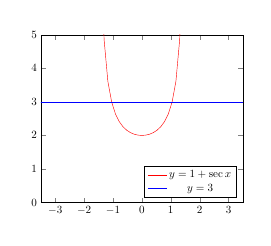
\begin{tikzpicture}[scale=0.4]
        \begin{axis}[ymin=0,ymax=5,xmin=-3.5,xmax=3.5,legend entries={$y=1+\sec x$, $y=3$},legend pos=south east]
\addplot [red,
domain=-pi/2:pi/2,
] {1+1/cos(deg(x))};
\addplot [blue,
domain=-4:4,
] {3};
\end{axis}
\end{tikzpicture}
\end{minipage}

\footnotesize
\pause
\begin{flalign*}
    V&=\int_{-\pi/3}^{\pi/3}\left(\pi(\textcolor{blue}3-1)^2 - \pi(\textcolor{red}{1+\sec x}-1)^2\right)\,dx=\pi\int_{-\pi/3}^{\pi/3}(4-\sec^2 x)\,dx\\
     &=\pi\left[4x-\tan x\right]_{-\pi/3}^{\pi/3}=\pi(4\pi/3-\sqrt3)-\pi(-4\pi/3+\sqrt3)=\boxed{\frac{8\pi^2}{3}-2\pi\sqrt3.}
\end{flalign*}
\pause (Note: we could have used symmetry to make the integral easier.)
\end{frame}

\begin{frame}{Volumes of solids of revolution (cylindrical shells)}
    Sometimes it is (much) easier to compute volumes of solids of revolution as follows.

    \vspace{2mm}
    \pause
    \textbf{Question}: find the volume of the solid of revolution obtained by rotating the region bounded by the curves $y=\sqrt{5+x^2}$, $y=0$, $x=0$ and $x=2$ around the $y$-axis.

    \vspace{2mm}
    \pause
    \textbf{Solution}: on the board (answer is $\frac23\pi(27-5^{3/2})$).
\end{frame}

\begin{frame}{Sample question (slide 1)}
    Let $f(x)=2xe^{2x}$.
    \begin{itemize}
        \item (a) Find the $x$- and $y$-coordinates of the local minima and maxima of $f(x)$.
        \item (b) Find the range of $f(x)$ for $-1\leq x\leq2$.
        \item (c) Find the area between the $x$-axis and the graph of $f(x)$ for $-1\leq x\leq 2$.
    \end{itemize}
    
\end{frame}

\begin{frame}{Sample question (slide 2)}

{\small Let $f(x)=2xe^{2x}$.
    \begin{itemize}
        \item (question a) Find the $x$- and $y$-coordinates of the local extrema of $f(x)$.
        \pause\item Solution: we compute the derivative $f'(x)=2e^{2x}+4xe^{2x}$ and set it to zero, so \begin{flalign*}
            2e^{2x}+4xe^{2x}=0\\
            2e^{2x}(1+2x)=0
        \end{flalign*}
        \pause
        Since $2e^{2x}$ is never equal to zero, our only solution to $f'(x)=0$ is $x=-\frac{1}{2}$. The corresponding $y$-coordinate is $f(-\frac{1}{2})=2(-\frac{1}{2})\cdot e^{2(-\frac{1}{2})}={-\frac{1}{e}}$.\pause

        We see that $f'(-1)=-2e^{-2}<0$ and $f'(0)=2>0$, so (by the first derivative test) we have a minimum, with coordinates $\boxed{{\left(-\frac{1}{2},-\frac{1}{e}\right)}}$. 
    \end{itemize}
}
\end{frame}

\begin{frame}{Sample question (slide 3)}
    Let $f(x)=2xe^{2x}$.
    \begin{itemize}
        \item (question b) Find the range of $f(x)$ for $-1\leq x\leq2$.
        \item\pause Solution: from question (a), we know that this function has a minimum with the coordinates $\left(-\frac{1}{2},-\frac{1}{e}\right)$. This minimum lies within the domain $-1\leq x\leq2$. \pause We are also interested in the value of $f(x)$ at the bounds of the domain, so we compute $f(-1)=-2e^{-2}$ and $f(2)=4e^4$. We observe that $-\frac{1}{e}<-2e^{-2}<4e^4$, so the range for $-1\leq x\leq2$ is $\boxed{\left[-\frac{1}{e},4e^4\right]}$.
    \end{itemize}
    
\end{frame}

\begin{frame}{Sample question (slide 4)}
    Let $f(x)=2xe^{2x}$.
    \begin{itemize}
        \item (question c) Find the area between the $x$-axis and the graph of $f(x)$ for $-1\leq x\leq 2$.
        \pause\item Solution: first compute the antiderivative of $f(x)$ using integration by parts: \[\int f(x)dx=\int2xe^{2x}dx=xe^{2x}-\int e^{2x}dx=\left(x-\frac{1}{2}\right)e^{2x}+C\]\pause
        
        We see that $f(x)$ is negative for $x<0$ and positive for $x>0$, so we have to split up the integral (we do not want ``negative area").\pause

        Our answer then becomes \[\hspace{-11mm}\left|\int_{-1}^0 f(x)dx\right|+\left|\int_{0}^{2} f(x)dx\right|=\left|-\frac{1}{2}+\frac{3}{2}e^{-2}\right|+\left|\frac{3}{2}e^4+\frac{1}{2}\right|=\boxed{1+\frac{3}{2}\left(e^4-e^{-2}\right)}\]
    \end{itemize}
    
\end{frame}

%\iffalse

MIT License

Copyright (c) 2023 Aron Hardeman

Permission is hereby granted, free of charge, to any person obtaining a copy
of this software and associated documentation files (the "Software"), to deal
in the Software without restriction, including without limitation the rights
to use, copy, modify, merge, publish, distribute, sublicense, and/or sell
copies of the Software, and to permit persons to whom the Software is
furnished to do so, subject to the following conditions:

The above copyright notice and this permission notice shall be included in all
copies or substantial portions of the Software.

THE SOFTWARE IS PROVIDED "AS IS", WITHOUT WARRANTY OF ANY KIND, EXPRESS OR
IMPLIED, INCLUDING BUT NOT LIMITED TO THE WARRANTIES OF MERCHANTABILITY,
FITNESS FOR A PARTICULAR PURPOSE AND NONINFRINGEMENT. IN NO EVENT SHALL THE
AUTHORS OR COPYRIGHT HOLDERS BE LIABLE FOR ANY CLAIM, DAMAGES OR OTHER
LIABILITY, WHETHER IN AN ACTION OF CONTRACT, TORT OR OTHERWISE, ARISING FROM,
OUT OF OR IN CONNECTION WITH THE SOFTWARE OR THE USE OR OTHER DEALINGS IN THE
SOFTWARE.

\fi
\section{Differential equations (DEs)}
\subsection{First order differential equations}
\tableofcontents[currentsection,currentsubsection]
\begin{frame}{Linear first order differential equations}
    \begin{tcolorbox}[colback=blue!5,colframe=blue!75!black,title=Linear first order DE]
In order to solve the linear differential equation \[y'+P(x)y=Q(x)\]

multiply both sides by $e^{\int P(x)dx}$ (the integrating factor), rewrite using the product rule for derivatives, and integrate both sides.
\end{tcolorbox}
\begin{itemize}
    \item Question: solve $y'+2x y=x$
    \item Solution: next slide.
\end{itemize}
\end{frame}

\begin{frame}{Example: linear 1st order DEs}
    \begin{itemize}
        \item\pause Question: solve $y'+2x y=x$
        \item\pause Solution: the integrating factor is $e^{\int 2xdx}=e^{x^2}$ (the constant of integration in the exponent is omitted). So we multiply both sides of the DE by $e^{x^2}$ and obtain \[e^{x^2}y'+2xe^{x^2}y=xe^{x^2}\]
        Using the product rule for derivatives, this can be rewritten as \[\left[e^{x^2}y\right]'=xe^{x^2}\]
        We integrate both sides and obtain \[e^{x^2}y=\int xe^{x^2} dx = \frac{1}{2}e^{x^2}+C\vspace{-1.5mm}\]
        \vspace{-1.5mm}We can divide both sides by $e^{x^2}$ to find the solution $\boxed{y=\frac{1}{2}+Ce^{-x^2}}$
    \end{itemize}

\end{frame}

\begin{frame}{Separable first order differential equations}
    \begin{itemize}
        \item A \textbf{separable} first order differential equation is an equation where the x's and y's can be ``separated", thus the equation can be rewritten into the form $y'f(y)=g(x)$. The method to solve these is to rewrite that equation to the form $f(y)dy=g(x)dx$ and then integrate both sides $\int f(y)dy=\int g(x)dx$:
        \item\pause Question: $xyy'=x^2+1$
        \item\pause Solution: rewrite the equation into $ydy=\frac{x^2+1}{x}dx$ and integrate both sides: $\int ydy=\int\frac{x^2+1}{x}dx$\pause

        So we find $\frac{1}{2}y^2=\frac{1}{2}x^2+\ln\left|x\right|+C$ \pause
        
        So the final answer becomes $\boxed{y=\pm\sqrt{x^2+2\ln \left|x\right| + C_*}}$ where $C_*=2C$.
    \end{itemize}

\end{frame}


\subsection{Second order differential equations}
\tableofcontents[currentsection,currentsubsection]

\begin{frame}

\frametitle{(Linear) second order differential equations}


\begin{tcolorbox}[colback=blue!5,colframe=blue!75!black,title=General form]
Homogeneous: $ay''+by'+cy=0$

Non-homogeneous: $ay''+by'+cy=f(x)$

{\footnotesize (here we will only deal with the case that $a,b$ and $c$ are constant real numbers)}
\end{tcolorbox}

\pause
Example:
\[y''-8y'+15y=0\]

\end{frame}
\begin{frame}
\frametitle{Solving a homogeneous 2nd order DE: basic example}
Example:
$y''-8y'+15y=0$

\pause

First construct the corresponding quadratic equation and solve it:
\begin{flalign*}
&r^2-8r+15=0\\ 
&(r-3)(r-5)=0\\
&r=3 \lor r=5\\
\end{flalign*}

\pause
We have two distinct real roots (3 and 5), so the general solution of the DE is
\[\boxed{y=c_1e^{3x}+c_2e^{5x}}\hspace{10mm}\text{for any constants $c_1$ and $c_2$}\]
\end{frame}




\begin{frame}
\frametitle{``Algorithm" to solve the homogeneous case}
You have some DE which you want to solve:
$\pmb{ay''+by'+cy=0}$

\begin{itemize}
\item Step 1: construct the characteristic equation: $ar^2+br+c=0$\pause
\item Step 2: solve it (compute the roots/solutions $r_1$ and $r_2$)\pause
\item Step 3: use the following scheme to find your final answer:
\begin{exampleblock}{Solution cases for homogeneous 2nd order DE}
\begin{itemize}
\item Real (non-equal) roots: \hspace{8.7mm} $y_{(x)}=c_1e^{r_1 x}+c_2e^{r_2x}$
\item One real root: \hspace{22mm} $y_{(x)}=c_1e^{rx}+c_2xe^{rx}$
\item Case $r_{1,2}=\alpha\pm i\beta$: \hspace{14mm} $y_{(x)}=e^{\alpha x}[c_1\cos (\beta x)+ c_2 \sin (\beta x)]$

\end{itemize}
\end{exampleblock}

\end{itemize}

\end{frame}






\begin{frame}
\frametitle{Solving a homogeneous 2nd order DE: another example}
{\small Example:
$7y''-7y'+2y=0$

\pause

First construct the corresponding quadratic equation and solve it:
\begin{flalign*}
&7r^2-7r+2=0\\ 
&r_{1,2}=\frac{-(-7)\pm\sqrt{(-7)^2-4\cdot7\cdot2}}{2\cdot7}\\
&r_{1,2}=\frac{7\pm\sqrt{-7}}{14}\\
&r_{1,2}=\frac{1}{2}\pm i\frac{\sqrt{7}}{14}\\
\end{flalign*}

\pause
(Recall: Case $r_{1,2}=\alpha\pm i\beta$: \quad $y_{(x)}=e^{\alpha x}[c_1\cos (\beta x)+ c_2 \sin (\beta x)]$)

\pause
We have two complex roots, so the general solution of the DE is
\[{y=e^{\frac{1}{2} x}\left[c_1\cos\left(\frac{\sqrt{7}}{14} x\right) + c_2\sin\left(\frac{\sqrt{7}}{14} x\right)\right]}\hspace{7mm}\text{for any constants $c_1$ and $c_2$}\]
}
\end{frame}



\begin{frame}
\frametitle{Solving a homogeneous 2nd order DE: one more example}
Example:
$y''+16y'+64y=0$

\pause

First construct the corresponding quadratic equation and solve it:
\begin{flalign*}
&r^2+16r+64=0\\
&(r+8)^2=0\\
&r=-8
\end{flalign*}

\pause
We have just one root this time!

(Recall: in case there's just one root: $y_{(x)}=c_1e^{r x}+c_2xe^{rx}$)

\pause
Therefore the general solution is:
\[\boxed{y=c_1e^{-8x}+c_2\pmb{x}e^{-8x}}\hspace{10mm}\text{for any constants $c_1$ and $c_2$}\]
Beware: in case there is only one root, multiply the second term (xor the first term) with $x$!
\end{frame}


%\subsubsection{Non-homogeneous}
\begin{frame}
\frametitle{NON-homogeneous second order DEs}

\begin{tcolorbox}[colback=blue!5,colframe=blue!75!black,title=General form]
$\pmb{ay''+by'+cy=f(x)}$

{\small ($a,b$ and $c$ are constant real numbers)}
\end{tcolorbox}

Plan of attack:
\begin{itemize}
\pause\item Step 1: consider the complementary equation $ay''+by'+cy=\pmb{0}$ and compute it's solution $y_c$. {\small(This is easy as it's a homogeneous equation)}
\pause\item Step 2: find some particular solution $y_p$ to the original non-homogeneous equation
\pause\item Step 3: your general solution to the original equation is now $y=y_c+y_p$
\end{itemize}
The difficulty may be mostly in step 2.
\end{frame}

\begin{frame}
\frametitle{Non-homogeneous second order DEs: example 1 (part 1)}


\begin{itemize}
\item Question: find the general solution of the differential equation $7y''-7y'+2y=x^2+7$.
\pause\item Step 1: we had already found the complementary solution (to the equation $7y''-7y'+2y=0$) before: ${y_c=e^{\frac{1}{2} x}\left[c_1\cos\left(\frac{\sqrt{7}}{14} x\right) + c_2\sin\left(\frac{\sqrt{7}}{14} x\right)\right]}$ for any constants $c_{1,2}$.
\pause\item Step 2: we must find some particular solution. Since $x^2+7$ is a 2nd order polynomial, let's set our particular solution to $y_p=Ax^2+Bx+C$. We plug this in the DE in order to find $A,B$, and $C$. 
\pause So we have $y_p=Ax^2+Bx+C$, $y_p'=2Ax+B$ and $y_p''=2A$. Let's plug this in:
\end{itemize}
\end{frame}

\begin{frame}
\frametitle{Non-homogeneous second order DEs: example 1 (part 2)}


\begin{itemize}
\item We will plug $y_p=Ax^2+Bx+C$, $y_p'=2Ax+B$ and $y_p''=2A$ in the original DE ($7y''-7y'+2y=x^2+7$) to find $A$, $B$ and $C$ of the particular solution:
\[7(2A)-7(2Ax+B)+2(Ax^2+Bx+C)=x^2+7\]
\[(2A)x^2+(-14A+2B)x+(14A-7B+2C)=x^2+7\]

\pause This must hold for all $x$, so the coefficients of the polynomials on the left- and right-hand side, must be equal. So, we have $2A=1$, and $-14A+2B=0$, and $14A-7B+2C=7$. \pause From the first one, we find $A=\frac{1}{2}$, then from the second one we find $B=\frac{7}{2}$, after which the third one gives us $C=\frac{49}{4}$. \pause Thus, we've found a particular solution: $y_p=\frac{1}{2}x^2+\frac{7}{2}x+\frac{49}{4}$.
\end{itemize}
\end{frame}

\begin{frame}
\frametitle{Non-homogeneous second order DEs: example 1 (part 3)}


\begin{itemize}
\item Step 3: now that we have found the complementary solution ${y_c=e^{\frac{1}{2} x}\left[c_1\cos\left(\frac{\sqrt{7}}{14} x\right) + c_2\sin\left(\frac{\sqrt{7}}{14} x\right)\right]}$ and a particular solution $y_p=\frac{1}{2}x^2+\frac{7}{2}x+\frac{49}{4}$, we can simply add them up to obtain the general solution of $7y''-7y'+2y=x^2+7$:

\[\boxed{{y=e^{\frac{1}{2} x}\left[c_1\cos\left(\frac{\sqrt{7}}{14} x\right) + c_2\sin\left(\frac{\sqrt{7}}{14} x\right)\right]}+\frac{1}{2}x^2+\frac{7}{2}x+\frac{49}{4}}\]
for any constants $c_1$ and $c_2$.
\end{itemize}
\end{frame}

\begin{frame}
\frametitle{The method of undetermined coefficients (formal)}{\scriptsize
\begin{itemize}
    \item In the previous example, we had $x^2+7$ (a polynomial of order 2) on the right-hand side of the differential equation. So we guessed that a particular solution could be a polynomial of order 2 as well ($Ax^2+Bx+C$). In general:\pause

    \begin{tcolorbox}[colback=blue!5,colframe=blue!75!black,title=Method of undetermined coefficients (FORMAL)]
    We search a particular solution to the differential equation $ay''+by'+cy=f(x)$.

    Let $P_n(x)$ and $Q_n(x)$ and $R_n(x)$ denote polynomials of order $n$.
    \begin{itemize}
        \item If $f(x)=e^{kx}P_n(x)$, then try $y_p=e^{kx}Q_n(x)$.
        \item If $f(x)=e^{kx}P_n(x)\sin mx$ or $f(x)=e^{kx}P_n(x)\cos mx$, then try $y_p=e^{kx}Q_n(x)\cos mx + e^{kx}R_n(x)\sin mx$
    \end{itemize}
    If any term in your ``guess" is a solution to the complementary equation, then multiply your guess $y_p$ by $x$ (or $x^2$ if it's still the case). 
    
    Plug your $y_p$-guess in the DE in order to find the coefficients of $Q_n(x)$ and $R_n(x)$.
    
    
    \end{tcolorbox}
    In the previous example we had the first case (with $k=0$ such that $e^{kx}=1$).

    
\end{itemize}}
\end{frame}

\begin{frame}
\frametitle{The method of undetermined coefficients (examples)}{\footnotesize
\begin{itemize}
    \item We search a particular solution to $ay''+by'+cy=f(x)$.
    \item If $f(x)=x^3$ or $f(x)=10000x^3+x+12$, we would try $y_p=Ax^3+Bx^2+Cx+D$.
    \item If $f(x)=\sin 8x$ or $f(x)=137\cos 8x$, we would try $y_p=A\cos 8x + B\sin 8x$.
    \item If $f(x)=e^{7x}$ or $f(x)=39e^{7x}$, we would try $y_p=Ae^{7x}$.
    \item If $f(x)=xe^{8x}$ or $f(x)=xe^{8x}+e^{8x}$, we would try $y_p=(Ax+B)e^{8x}$.
    \item If $f(x)=x^2\sin {x}$, we would try $y_p=(Ax^2+Bx+C)\cos x + (Dx^2+Ex+F)\sin x$.
    \item If $f(x)=e^{9x}x^2\sin 4x$, we would try $y_p=e^{9x}(Ax^2+Bx+C)\cos 4x + e^{9x}(Dx^2+Ex+F)\sin 4x$.
    \item Notice that the last two examples are so long that you will probably not get them on your exam (since you'd have to solve for 6 coefficients). However they are useful as a demonstration of the principle.
    \item \textbf{Do not forget that you have to multiply your $y_p$-guess by $x$ if any term in your guess is a solution to the complementary equation.}
    
\end{itemize}}
\end{frame}

\begin{frame}{The superposition principle}
\[ay''+by'+cy=f_1(x)+f_2(x)\]
\begin{itemize}
    \item Sometimes, $f(x)$ is a sum of multiple functions, say $f(x)=f_1(x)+f_2(x)$. In that case, you can just find a particular solution $y_{p1}$ to the differential equation $ay''+by'+cy=f_1(x)$ and a particular solution $y_{p2}$ to the differential equation $ay''+by'+cy=f_2(x)$.

    \item Your particular solution to the differential equation $ay''+by'+cy=f_1(x)+f_2(x)$ is then given by $y_{p1}+y_{p2}$.
    \item Do not forget to add the complementary solution to your answer as well.

    \item (This also works for a sum of more than two functions; see next slide for a full example.)
    \end{itemize}
\end{frame}

\begin{frame}{Superposition principle \& method of u.c. (example)}

{\scriptsize
\begin{itemize}
    \item Question: solve $y''-6y'+8y=xe^{3x}+xe^{4x}+xe^{5x}$.
    \item The complementary solution is $\textcolor{teal}{y_c=c_1e^{2x}+c_2e^{4x}}$ for any constants $c_1$ and $c_2$.
    \item Let $\textcolor{red}{y_{p1}}$ be a particular solution to $y''-6y'+8y=xe^{3x}$. Then $\textcolor{red}{y_{p1}}$ must be of the form $\textcolor{red}{y_{p1}=(Ax+B)e^{3x}}$. Substituting this in $y''-6y'+8y=xe^{3x}$ gives that $A=-1$ and $B=0$. So we find $\textcolor{red}{y_{p1}=-xe^{3x}}$.
    \item Let $\textcolor{blue}{y_{p2}}$ be a particular solution to $y''-6y'+8y=xe^{4x}$. Then $\textcolor{blue}{y_{p2}}$ would be of the form $\textcolor{gray}{y_{p2}=(Cx+D)e^{4x}}$, but we observe that the term $De^{4x}$ is a solution to the complementary equation (since $y_c=c_1e^{2x}+c_2e^{4x}$), thus we multiply the $\textcolor{blue}{y_{p2}}$-guess by $x$ and obtain $\textcolor{blue}{y_{p2}=(Cx^2+Dx)e^{4x}}$. We substitute this into $y''-6y'+8y=xe^{4x}$ and obtain $C=\frac{1}{4}$ and $D=-\frac{1}{4}$, so we find $\textcolor{blue}{y_{p2}=(\frac{1}{4}x^2-\frac{1}{4}x)e^{4x}}$.
    \item Let $\textcolor{violet}{y_{p3}}$ be a particular solution to $y''-6y'+8y=xe^{5x}$. Then $\textcolor{violet}{y_{p3}}$ must be of the form $\textcolor{violet}{y_{p3}=(Ex+F)e^{5x}}$. Substituting this in $y''-6y'+8y=xe^{5x}$ gives that $E=\frac{1}{3}$ and $F=-\frac{4}{9}$. So we find $\textcolor{violet}{y_{p3}=(\frac{1}{3}x-\frac{4}{9})e^{5x}}$.
    \item The particular solution to the original differential equation is now $\textcolor{red}{y_{p1}}+\textcolor{blue}{y_{p2}}+\textcolor{violet}{y_{p3}}=\textcolor{red}{-xe^{3x}}+\textcolor{blue}{(\frac{1}{4}x^2-\frac{1}{4}x)e^{4x}}+\textcolor{violet}{(\frac{1}{3}x-\frac{4}{9})e^{5x}}$. We add the full particular solution to the complementary solution and obtain as our final answer:
    \[\boxed{y=\textcolor{teal}{c_1e^{2x}+c_2e^{4x}}\textcolor{red}{-xe^{3x}}\textcolor{blue}{+\left(\frac{1}{4}x^2-\frac{1}{4}x\right)e^{4x}}\textcolor{violet}{+\left(\frac{1}{3}x-\frac{4}{9}\right)e^{5x}}}\qquad\text{for all $c_1$ and $c_2$}\]
    \end{itemize}
}\end{frame}

\begin{frame}
\frametitle{Sample question on differential equations (slide 1)}
\textbf{Question:} solve the initial value problem \[y''+2y'-35y=3e^{5x}\qquad y(0)=137\qquad y'(0)=42\]

\textbf{Solution steps:}
\begin{itemize}
    \item\pause Step 1: solve the homogeneous equation $y''+2y'-35y=0$ to find the complementary solution.
    \item\pause Step 2: use the method of undetermined coefficients to find a particular solution to the original (non-homogeneous) equation.
    \item\pause Step 3: we add the complementary solution to the particular solution to find the general solution of the original equation.
    \item\pause Step 4: apply the initial values to obtain the final answer.
    \item\pause (Fully worked out solution on next slides)
\end{itemize}
\end{frame}

\begin{frame}{Sample question on differential equations (slide 2)}
    \textbf{Question:} solve the initial value problem \[y''+2y'-35y=3e^{5x}\qquad y(0)=137\qquad y'(0)=42\]
    
    \textbf{Step 1:} first we solve $y''+2y'-35y=0$. \pause The characteristic equation is $r^2+2r-35=0$, thus $(r+7)(r-5)=0$, so the roots are $5$ and $-7$, two distinct real numbers.\pause

    Thus, the complementary solution takes the form $y_c = c_1e^{5x} + c_2e^{-7x}$ for any constants $c_1$ and $c_2$. (Later we will determine which $c_1$ and $c_2$ suit our initial values.)
\end{frame}

\begin{frame}{Sample question on differential equations (slide 3)}
    \textbf{Question:} solve the initial value problem \[y''+2y'-35y=3e^{5x}\qquad y(0)=137\qquad y'(0)=42\]
    
    \textbf{Step 2:} we apply the method of undetermined coefficients as explained before. $f(x)=3e^{5x}$, so we would try the particular solution $\textcolor{gray}{y_p=Ae^{5x}}$.
    \begin{itemize}
    \item{\scriptsize(Recall the first case from the method of u.c.: if $f(x)=e^{kx}P_n(x)$, then try $y_p=e^{kx}Q_n(x)$. Here $P_n(x)=3$, a ``polynomial" of degree 0)}
    \end{itemize}\pause
    However, the complementary solution was $y_c = c_1e^{5x} + c_2e^{-7x}$ for any constants $c_1$ and $c_2$. We observe that our trial particular solution $\textcolor{gray}{y_p=Ae^{5x}}$ will not work, because it is a solution to the complementary equation! Thus, we multiply our guess by $x$, so our trial particular solution is $\pmb{y_p=Axe^{5x}}$, but we still need to find the constant $A$ (next slide).

\end{frame}

\begin{frame}{Sample question on differential equations (slide 4)}
    \textbf{Question:} solve the initial value problem \[y''+2y'-35y=3e^{5x}\qquad y(0)=137\qquad y'(0)=42\]
    
    \textbf{Step 2 (continuation):} our trial particular solution is $y_p=Axe^{5x}$, but we need to find $A$. So we compute the derivatives: $y_p'=A(e^{5x}+5xe^{5x})$ and $y_p''=A(5e^{5x}+5e^{5x}+25xe^{5x})=A(10e^{5x}+25xe^{5x})$\pause

    We substitute this in the original differential equation to find: \[A(10e^{5x}+25xe^{5x})+2A(e^{5x}+5xe^{5x})-35Axe^{5x}=3e^{5x}\] \vspace{-7mm}\[\iff 12Ae^{5x}=3e^{5x}\]\pause
    So we take $A=\frac{1}{4}$. The guess worked (since we were able to find an $A$ such that $y_p=Axe^{5x}$ satisfies the differential equation), so we found the valid particular solution $\pmb{y_p=\frac{1}{4}xe^{5x}}$.

    

\end{frame}




\begin{frame}{Sample question on differential equations (slide 5)}
    \textbf{Question:} solve the initial value problem \[y''+2y'-35y=3e^{5x}\qquad y(0)=137\qquad y'(0)=42\]
    
    \textbf{Step 3):} the general solution to the complementary equation was $y_c = c_1e^{5x} + c_2e^{-7x}$ and a particular solution is $y_p=\frac{1}{4}xe^{5x}$. We add these together to obtain the general solution to the non-homogeneous (original) equation for any constants $c_1$ and $c_2$:\pause

    \[y=c_1e^{5x} + c_2e^{-7x} +\frac{1}{4}xe^{5x}\]\pause

    This is a solution for every $c_1$ and $c_2$, but we were given an initial value problem, i.e. we still have to find $c_1$ and $c_2$ such that $y(0)=137$ and $y'(0)=42$ (step 4, next slide).
    

\end{frame}


\begin{frame}{Sample question on differential equations (slide 6)}
    \textbf{Question:} solve the initial value problem \[y''+2y'-35y=3e^{5x}\qquad y(0)=137\qquad y'(0)=42\]
    
    \textbf{Step 4):} the general solution to the differential equation is
    $y=c_1e^{5x} + c_2e^{-7x} +\frac{1}{4}xe^{5x}$\pause, with derivative $y'=5c_1e^{5x}-7c_2e^{-7x}+\frac{1}{4}e^{5x}+\frac{5}{4}xe^{5x}$.

    We need to have $y(0)=137$ and $y'(0)=42$\pause, i.e.
    \[y(0)=c_1+c_2=137\qquad y'(0)=5c_1-7c_2+\frac{1}{4}=42\]\pause
    Substituting $c_2=137-c_1$ into the second equation gives $5c_1-7(137-c_1)+\frac{1}{4}=42 \iff 12c_1=\frac{4003}{4} \iff c_1=\frac{4003}{48}$ and from we first equation we obtain $c_2=137-\frac{4003}{48}=\frac{2573}{48}$. Therefore, the solution is \[\boxed{\boxed{y=\frac{4003}{48}e^{5x} + \frac{2573}{48}e^{-7x} +\frac{1}{4}xe^{5x}}}\]

    

\end{frame}



\begin{frame}
	\frametitle{Method of variation of constants}{\scriptsize
        We already discussed the method of undetermined coefficients to solve nonhomogeneous linear ODEs. Now we discuss another method: \textbf{variation of constants} (or \textbf{variation of parameters}).

		\pause Suppose we have the general solution $y(x)=c_1y_1(x)+c_2y_2(x)$
		to some \textit{homogeneous} DE $ay''+by'+cy=0$.
		\begin{itemize}
			\pause	\item Then we can replace the constants $c_1$, $c_2$ by functions $u_1(x)$ and $u_2(x)$, and try to find a \textit{particular} solution to the \textit{nonhomogeneous} equation $ay''+by'+cy=f(x)$ of the form
			      \[y_p(x)=u_1(x)y_1(x)+u_2(x)y_2(x)\]
			      %\pause\item To make calculations easier, we impose the constraint that \[u_1'y_1 + u_2'y_2=0\]

			      \pause\item Then we solve this system of equations for $u_1'$ and $u_2'$:
			      $$\begin{cases}a(u_1'y_1'+u_2'y_2')=f\qquad&\text{\color{orange!50!red}(this comes from subbing $y_p$ into the DE)}\\u_1'y_1 + u_2'y_2=0&\text{\color{orange!50!red}(this is an additional constraint we impose!)}\end{cases}$$
			      \pause\item Then we integrate $u_1'$ and $u_2'$ to find $u_1$ and $u_2$, and then we found the general solution to the nonhomogeneous equation.
			      \pause\item Note: this method can be extended to many more types of equations, e.g. equations with nonconstant coefficients. This is helpful if you have to find the general solution given some particular solutions.
		\end{itemize}}
\end{frame}

\begin{frame}
	\frametitle{Variation of constants: condensed example}{\small
	\textbf{Question}: solve $y''+3y'+2y=\sin(e^x)$.

	\pause\textbf{Solution}: a general solution to the equation $y''+3y'+2y=0$ is given by $y(x)={\color{lime!50!black}c_1e^{-x}+c_2e^{-2x}}$. Now we have to solve the system of equations\pause
	\[\begin{cases}-u_1'e^{-x} -2u_2'e^{-2x}=\sin(e^x) \qquad\text{\color{orange!50!red}(note that $a=1$)}\\u_1'e^{-x}+u_2'e^{-2x}=0\end{cases}\]
	\pause Adding the two rows together, we find $-u_2'e^{-2x}=\sin(e^x)$, so $u_2'=-e^{2x}\sin(e^x)$. \pause{}Then, we can also find $u_1'=e^x\sin(e^x)$.

	\pause Both integrals can be solved by substituting $t=e^x$ (then $dt=e^xdx$):
	\pause\begin{flalign*}
		u_1(x) & =-\cos(e^x)                                                             \\
		u_2(x) & =e^x\cos(e^x)-\sin(e^x)\qquad\text{(omitting constants of integration)}
	\end{flalign*}
	\pause So a particular solution to the nonhomogeneous equation is $y_p(x)=-\cos(e^x)e^{-x}+(e^x\cos(e^x)-\sin(e^x))e^{-2x}={\color{red}-e^{-2x}\sin(e^x)}$. \pause{}So the general solution is
	\[\boxed{y(x)={\color{lime!50!black}c_1e^{-x}+c_2e^{-2x}}\, {\color{red} -e^{-2x}\sin(e^x)}}\]
	}\end{frame}

\begin{frame}
	\frametitle{Extra: constructing an ODE from its solutions}{\small
		\begin{itemize}
			\item\textbf{Question}: give a linear homogeneous ODE with constant coefficients of minimal order, which admits the solutions $y_1=42\cos x$, $y_2=-x\cos x$ and $y_3=e^{42x}$.

			\pause\item\textbf{Solution}: think backwards. If $y_1$, $y_2$ and $y_3$ are solutions, they must correspond to roots in the characteristic equation of the ODE.
			\pause\item The solution $42\cos x$ corresponds to the roots $r=\pm i$. \pause{}As $-x\cos x$ must also be a solution, these roots must both occur with multiplicity two.

			      \pause\item The solution $e^{42x}$ corresponds to the root $r=42$.

			      \pause\item So the characteristic equation must be $$(r^2+1)^2(r-42)=0$$
			      \item\pause Expanding brackets and replacing powers of $r$ by derivatives of $y$, we find the answer
                      \[\boxed{y'''''-42y''''+2y'''-84y''+y'-42y=0}\]
		\end{itemize}

	}
\end{frame}







































\iffalse

\begin{frame}{Sample question on differential equations (slide 2)}
    \textbf{Question:} solve the initial value problem \[y''+2y'-35y=3e^{3x}\qquad y(0)=137\qquad y'(0)=42\]
    
    \textbf{Step 1:} first we solve $y''+2y'-35y=0$. The characteristic equation is $r^2+2r-35=0$, thus $(r+7)(r-5)=0$, so the roots are $-5$ and $7$, two distinct real numbers.

    Thus, the complementary solution takes the form $y_c = c_1e^{-5x} + c_2e^{7x}$ for any constants $c_1$ and $c_2$. (Later we will determine which $c_1$ and $c_2$ suit our initial values.)
\end{frame}

\begin{frame}{Sample question on differential equations (slide 3)}
    \textbf{Question:} solve the initial value problem \[y''+2y'-35y=3e^{3x}\qquad y(0)=137\qquad y'(0)=42\]
    
    \textbf{Step 2:} we apply the method of undetermined coefficients as explained before. $f(x)=3e^{3x}$, so we would try the particular solution $y_p=Ae^{3x}$.
    \begin{itemize}
    \item{\scriptsize(Recall the first case from the method of u.c.: if $f(x)=e^{kx}P_n(x)$, then try $y_p=e^{kx}Q_n(x)$. Here $P_n(x)=3$, a ``polynomial" of degree 0)}
    \end{itemize}
    The derivatives are $y_p'=3Ae^{3x}$ and $y_p''=9Ae^{3x}$, and we plug this in the differential equation to obtain
    \[9Ae^{3x}+2(3Ae^{3x})-35Ae^{3x}=3e^{3x}\iff-20Ae^{3x}=3e^{3x}\]
    So we take $A=-\frac{3}{20}$, (our guess worked,) thus we found a valid particular solution $\pmb{y_p=-\frac{3}{20}e^{3x}}$.

\end{frame}

\begin{frame}{Sample question on differential equations (slide 4)}
    \textbf{Question:} solve the initial value problem \[y''+2y'-35y=3e^{3x}\qquad y(0)=137\qquad y'(0)=42\]
    
    \textbf{Step 3:} we add the complementary solution to the particular solution and obtain as the general solution to the differential equation: \[y=c_1e^{-5x} + c_2e^{7x}-\frac{3}{20}e^{3x}\] for any constants $c_1$ and $c_2$. However, the question was an initial value problem; we still have to determine $c_1$ and $c_2$ such that the initial values hold.

\end{frame}

\begin{frame}{Sample question on differential equations (slide 5)}
    \textbf{Question:} solve the initial value problem \[y''+2y'-35y=3e^{3x}\qquad y(0)=137\qquad y'(0)=42\]
    
    \textbf{Step 4:} we have the general solution and compute its derivative: \[y(x)=c_1e^{-5x} + c_2e^{7x}-\frac{3}{20}e^{3x}\]  \vspace{-5mm}\[y'(x)=-5c_1e^{-5x}+7c_2e^{7x}-\frac{9}{20}e^{3x}\]
    We apply the initial conditions: \[y(0)=c_1+c_2-\frac{3}{20}=137\quad\quad y'(0)=-5c_1+7c_2-\frac{9}{20}=42\]
    

\end{frame}
\fi

\iffalse

MIT License

Copyright (c) 2023 Aron Hardeman

Permission is hereby granted, free of charge, to any person obtaining a copy
of this software and associated documentation files (the "Software"), to deal
in the Software without restriction, including without limitation the rights
to use, copy, modify, merge, publish, distribute, sublicense, and/or sell
copies of the Software, and to permit persons to whom the Software is
furnished to do so, subject to the following conditions:

The above copyright notice and this permission notice shall be included in all
copies or substantial portions of the Software.

THE SOFTWARE IS PROVIDED "AS IS", WITHOUT WARRANTY OF ANY KIND, EXPRESS OR
IMPLIED, INCLUDING BUT NOT LIMITED TO THE WARRANTIES OF MERCHANTABILITY,
FITNESS FOR A PARTICULAR PURPOSE AND NONINFRINGEMENT. IN NO EVENT SHALL THE
AUTHORS OR COPYRIGHT HOLDERS BE LIABLE FOR ANY CLAIM, DAMAGES OR OTHER
LIABILITY, WHETHER IN AN ACTION OF CONTRACT, TORT OR OTHERWISE, ARISING FROM,
OUT OF OR IN CONNECTION WITH THE SOFTWARE OR THE USE OR OTHER DEALINGS IN THE
SOFTWARE.

\fi
\section{Taylor polynomials}
\tableofcontents[currentsection,currentsubsection]
\begin{frame}{Taylor polynomials}
    Sometimes, we want to approximate a function by a polynomial.

    The $n$th degree \emph{Taylor polynomial} of function $f$ at $x=a$ is given by
    \[T_n(x)=\sum_{j=0}^n\frac{f^{(j)}(a)}{j!}(x-a)^j,\]
    provided $f$ is differentiable $n$ times.

    \color{gray}This definition has been chosen such that the $i$th derivatives of $f$ are equal to the $i$th derivatives of $T_n(x)$ for $i\in\{0,1,\dots,n\}$. Intuitively, this ensures that around $x=a$, the behavior of the polynomial is similar to the behavior of $f$, i.e., the polynomial \emph{approximates} $f$.
\end{frame}

\begin{frame}
\frametitle{Visualization}
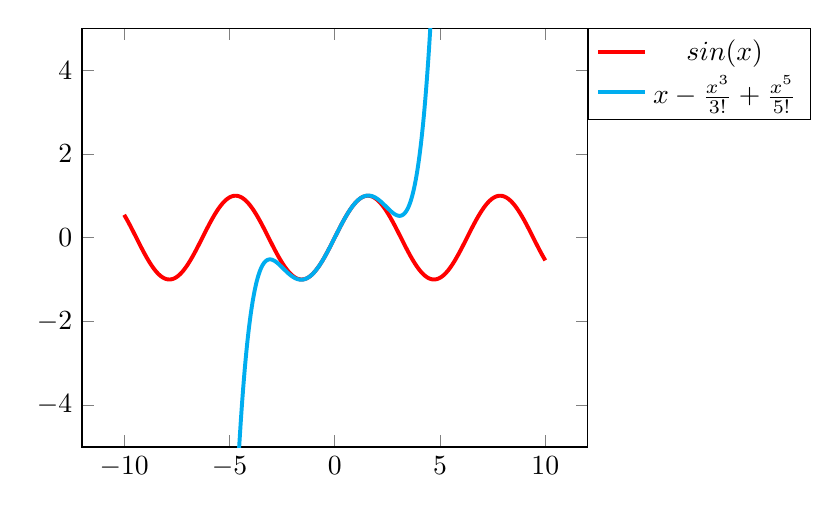
\begin{tikzpicture}
\begin{axis}[legend style={at={(1,1)},anchor=north west},ymin=-5, ymax=5]
\addplot[line width=0.5mm,color=red, domain=-10:10, samples=500]{sin(deg(x))};
\addlegendentry{\(sin(x)\)}
%\addplot[color=blue, domain=-10:10, samples=500]{x};
%\addlegendentry{\(x\)}
%\addplot[color=green, domain=-10:10, samples=500]{x-((x^3)/(3!))};
%\addlegendentry{\(x-\frac{x^3}{3!}\)}
\addplot[line width=0.5mm,color=cyan, domain=-5:5, samples=500]{x-((x^3)/(3!))+((x^5)/(5!))};
\addlegendentry{\(x-\frac{x^3}{3!}+\frac{x^5}{5!}\)}
%\addplot[color=black, domain=-7:7, samples=500]{x-((x^3)/(3!))+((x^5)/(5!))-((x^7)/(7!))};
%\addlegendentry{\(\mathsmaller{{x-\frac{x^3}{3!}+\frac{x^5}{5!}-\frac{x^7}{7!}}}\)}
\end{axis}
\end{tikzpicture}

{ Interactive version: \url{https://www.desmos.com/calculator/elb2sjyuhu}}
\end{frame}


\begin{frame}
\frametitle{Example Taylor polynomial question}
{\scriptsize
    Find an expression for the $(2n+1)$th degree Taylor polynomial $T_{2n+1}(x)$ of the function $f(x)=\sin x$ centered around $x=0$.

------------------------------------------------------------------------------

\pause
Solution: let's compute some derivatives:
\[f^{(0)}(x)=f(x)=\sin x\quad\quad\quad\quad f^{(0)}(0)=0\]
\vspace*{-\baselineskip}\pause\[f^{(1)}(x)=\cos x\quad\quad\quad\quad f^{(1)}(0)=1\]
\vspace*{-\baselineskip}\pause\[f^{(2)}(x)=-\sin x\quad\quad\quad\quad f^{(2)}(0)=0\]
\vspace*{-\baselineskip}\pause\[f^{(3)}(x)=-\cos x\quad\quad\quad\quad f^{(3)}(0)=-1\]
\vspace*{-\baselineskip}\pause\[f^{(4)}(x)=\sin x\quad\quad\quad\quad f^{(4)}(0)=0\]
\vspace*{-\baselineskip}\pause\[f^{(5)}(x)=\cos x\quad\quad\quad\quad f^{(5)}(0)=1\]

\pause We see a pattern! These derivatives will infinitely repeat in a cycle of length four. Using the definition, we get
\begin{flalign*}T_{2n+1}(x)&=\sum_{j=0}^{2n+1}\frac{f^{(j)}(a)}{j!}(x-a)^j=\sum_{j=0}^{2n+1}\frac{f^{(j)}(0)}{j!}x^j\\
    &=x-\frac{x^3}{3!}+\frac{x^5}{5!}-\dots+(-1)^n\frac{x^{2n+1}}{(2n+1)!}=\boxed{\sum_{i=0}^{n}\frac{(-1)^ix^{2i+1}}{(2i+1)!}}.
\end{flalign*}

}
\end{frame}

\begin{frame}{Evaluating limits with Taylor polynomials}
    \begingroup
    \scriptsize
    We can do some nice things with Taylor polynomials, such as evaluating limits.

    \begin{itemize}
        \item \textbf{Question}: evaluate $\displaystyle\lim_{x\to0}\frac{(\sin\sqrt x)^2-x\cos x+\frac13x^2}{x\ln(1+x)-x^2}.$
        \item \textbf{Solution}: replace some of the terms by their Taylor polynomial:
    \end{itemize}
    \vspace{-3mm}
            \begin{flalign*}
                \lim_{x\to0}&\frac{{\color{red}(\sin\sqrt x)^2}-{\color{blue}x\cos x}+\frac13x^2}{\color{teal!30!green}x\ln(1+x)\color{black}-x^2}\\
                            &=\lim_{x\to0}\frac{{\color{red}\left[x^{1/2}-\frac{x^{3/2}}{3!}+\frac{x^{5/2}}{5!}+O(x^{7/2})\right]^2}-{\color{blue}x\left[1-\frac{x^2}{2!}+O(x^4)\right]}+\frac13x^2}{\color{teal!30!green}x\left[x-\frac{x^2}2+O(x^3)\right]\color{black}-x^2}\\
                            %&\qquad\color{orange}\text{(do this step on the board)}\\
                             &=\lim_{x\to0}\frac{{\color{red}\left[x-\frac13 x^2+(\frac1{3!3!}+\frac{2}{5!})x^3+O(x^4)\right]}-{\color{blue}\left[x-\frac{x^3}{2!}+O(x^5)\right]}+\frac13x^2}{{\color{teal!30!green}\left[x^2-\frac{x^3}2+O(x^4)\right]}-x^2}\\
                             &=\lim_{x\to0}\frac{(\frac1{3!3!}+\frac{2}{5!}+\frac1{2!})x^3+O(x^4)}{-\frac{1}2x^3+O(x^4)}=\lim_{x\to0}\frac{\frac{49}{90}+O(x)}{-\frac12+O(x)}=\frac{\frac{49}{90}+0}{-\frac12+0}=\boxed{-\frac{49}{45}}.
            \end{flalign*}
        \textbf{Note: in a similar fashion, you can approximate integrals using Taylor polynomials.}
    \endgroup
\end{frame}

\begin{frame}{Taylor's theorem}
    \begingroup
    \small
    Let us write $f(x) = T_n(x) + E_n(x)$, where $T_n(x)$ is the $n$th degree Taylor polynomial of the function $f$ around $x=a$. We call $E_n(x)$ the \emph{error term}.

    \begin{tcolorbox}[title=Taylor's theorem ,colback=yellow!50,colframe=violet!85!black]
    If $f$ is $n+1$ times differentiable on the open interval between $a$ and $x$ and $f^{(n)}$ is continuous on the closed interval between $a$ and $x$, then
    \[E_n(x)=\frac{f^{(n+1)}(c)}{(n+1)!}(x-a)^{n+1}\]
    for some $c$ between $a$ and $x$.
    \end{tcolorbox}
    Error estimation theorem (corollary): if there is a positive constant $M$ for which $|f^{(n+1)}(y)|\leq M$ for all $y$ between $a$ and $x$, then
    \[|E_n(x)|\leq \frac{M|x-a|^{n+1}}{(n+1)!}.\]
    \endgroup
\end{frame}

\begin{frame}{Error estimation using Taylor's theorem}
    \textbf{Question}: estimate $\sin(1^\circ)$ with an error less than $10^{-18}$.

    \vspace{2mm}
    \textbf{Solution}: 
    \begin{itemize}
        \item We want to approximate $\sin(1^\circ)=\sin\frac1{360}$ using the Taylor polynomials of $\sin x$ (centered around $x=0$). So, for which $n$ do we have $|E_n(\frac1{360})|<10^{-18}$?

        \item By the Error estimation theorem with $M=1$ (why?), we find that $|E_n(\frac1{360})|<10^{-18}$ whenever $\frac{(\frac1{360})^{n+1}}{(n+1)!}<10^{-18}$. This holds for $n\geq5$.

        \item Hence, it suffices to use the Taylor polynomial of degree $5$. We get
            {\footnotesize\[\sin(1^\circ)\approx (1/360)-\frac{(1/360)^3}6+\frac{(1/360)^5}{120}={\color{green!70!teal}0.002777774205534071}367988\dots\]}

        \item Verification: {\footnotesize$\sin(\frac1{360})={\color{green!70!teal}0.002777774205534071}367734\dots$}
        
            Verdict: success!

        \end{itemize}
    
\end{frame}







\end{document}
